\documentclass[../CMPUT-404-Notes.tex]{subfiles}
\begin{document}
\chapter{Websockets}
\section{Websockets}
\textbf{Webscokets} is a computer communications protocol, providing full-duplex communication channels over a single TCP connection. It can work on HTTP which is a good thing because JavaScript in the browser can't do TCP or UDP. 

\begin{DndSidebar}[color=PhbLightGreen]{HTTP}
    \begin{itemize}
        \item Traditionally, you make a request and get a response 
        \item Problem: Not nearly as flexible as UDP and TCP
        \item Workarounds:
        \begin{itemize}
            \item Polling
            \item Long-polling (Comet)
            \item Other tricks
        \end{itemize}
    \end{itemize}
\end{DndSidebar}

We want to send messages either way whenever, we want them to arrive in order, the primary solution is to \textbf{Websockets}. \textbf{WebRTC} and \textbf{EventSource} are also valid solutions but less common. 


\subsubsection{Technology Breakdown}
\begin{itemize}
    \item Websockets!
    \begin{itemize}
        \item Messages
        \item Full duplex
    \end{itemize}
    \item WebRTC
    \begin{itemize}
        \item Streaming Media
        \item Messages (same API as Websockets)
    \end{itemize}
    \item EventSource
    \begin{itemize}
        \item Sever-generated events
        \item Just HTTP
    \end{itemize}
\end{itemize}

You can upgrade existing HTTP connections to a websockets by using the \texttt{Upgrade} header. 
This allows websockets to operate on the same port as HTTP(S) and allows them to be compatible with proxies and reverse proxies. 

\subsection{Why Websockets}
It allows for full-duplex message-based communication
\begin{itemize}
    \item Server can push whenever, client can push whenever
    \item Both sides can send data at the same time
    \item Connection stays open
    \item Don't need to poll
    \item Avoid big HTTP headers for each message
    \item Reuse existing technologies as much as possible
\end{itemize}

\subsection{Websocket Handshake}
First the client makes a request
\begin{minted}[breaklines]{http}
GET /chat HTTP/1.1
Host: server.example.com
Upgrade: websocket
Connection: Upgrade
Sec-WebSocket-Key: dGhlIHNhbXBsZSBub25jZQ==
Origin: http://example.com
Sec-WebSocket-Protocol: soap, wamp
Sec-WebSocket-Version: 13   
\end{minted}
And the server responses with 
\begin{minted}[breaklines]{http}
HTTP/1.1 101 Switching Protocols
Upgrade: websocket
Connection: Upgrade
Sec-WebSocket-Accept: s3pPLMBiTxaQ9kYGzzhZRbK+xOo=
Sec-WebSocket-Protocol: wamp
\end{minted}
Use GET to specify which Websocket, 1 webserver can service multiple websocket services. 
\textit{wss://server.example.com/mysocket}.
\texttt{Connection: Upgrade} is used to upgrade the connection to use websockets not \texttt{keep-alive} nor \texttt{close}.
\texttt{Upgrade: websocket} specifiy the protocol we're upgrading to.
An optional header can be sent, \texttt{Sec-WebSocket-Protocol: wamp}, this specify the sub-protocol on what kind of websockets the user agent want to use.

\subsubsection{Key and Accept}
It uses a kind of Brown M\&M test. The client sends \texttt{Sec-WebSocket-Key} with a random string. 
The server responses with a \texttt{Sec-WebSocket-Accept} header. This header is generated by taking the client key and appends, \texttt{258EAFA5-E914-47DA-95CA-C5AB0DC85B11}. Then takes the SHA1 sum of the appended key. Then finally takes the base64-encoding of the SHA1 sum to generate the accept.
After this the client knows for sure the server's ready for websocket.

\section{Websocket Protocol}
The client and server exchange "frames".
\begin{itemize}
    \item The control frames (out of band): with the hex code \texttt{0x8} to close the connection, \texttt{0x9} for a ping and \texttt{0xA} for a pong. 
    \item The data frame: These are the messages, updates, events, RPCs, whatever you're exchanging with the server.    
\end{itemize}

\subsection{Messages}
Are sent in data frames, the messages could be binary or text, and the size if known ahead of time. This allows for efficient buffering.
The messages could be fragmented into multiple data frames.

\begin{figure}[!h]
    \centering
    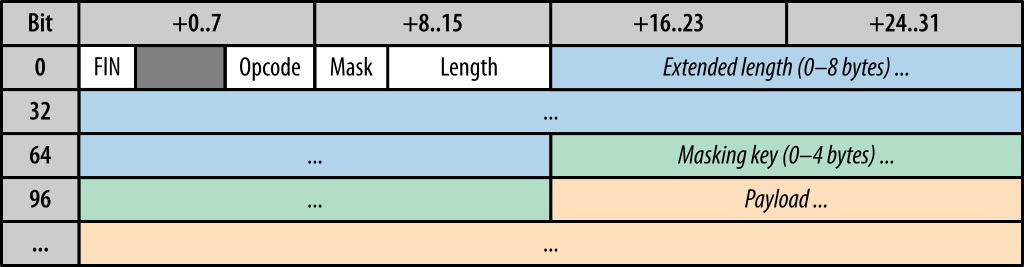
\includegraphics[width=\columnwidth]{../assets/websocket-frame.png}
    \caption{Websocket Format}
    \label{fig:websocket}
\end{figure}

In \Cref{fig:websocket} shows the websocket format.

The first byte contains
\begin{itemize}
    \item \texttt{FIN} bit 
    \item 3 reserved bits 
    \item 4-bit opcode  
\end{itemize} 
The second byte contains:
\begin{itemize}
    \item A mask bit that enables XOR "encryption" mask 
    \item 7-bits for payload length.
    \item If the payload length = 126 then a 16-bit payload length follows
    \item If the payload length = 127 then a 64-bit payload length follows
    \item If masks is set then the masking key follows
\end{itemize}
Finally the data.
\\~\\
The smallest fragment is a one byte message, no mask equals 4 bytes. 
The largest possible header is 14 bytes.
Each message just send fragments until FIN.
Ordering is handled by TCP. 

\subsection{Opcodes}
There are several opcodes for websockets
\begin{itemize}
    \item \texttt{0x1} UTF-8 text (don't break characters)
    \item \texttt{0x2} binary
    \item \texttt{0x8} close
    \item \texttt{0x9} ping
    \item \texttt{0xa} pong
\end{itemize}

\subsubsection{Example}
\mintinline{text}{0x01 0x03 0x48 0x65 0x6c} => "Hel".
The \texttt{0x01} tells the recipient, that the message is UTF-8. 
The \texttt{0x03} is the payload length of 3.
\mintinline{text}{0x80 0x02 0x6c 0x6f} => "lo".
The \texttt{0x80} sets the FIN bit and nothing else.
The \texttt{0x02} is the payload length of 2.

\subsection{Why the mask}
The primary reason for the mask is to prevent accidentally being parsed as HTTP. 
The websocket protocol is supposed to work with existing infrastructure and maintainers were worried about cache poisoning by sending fake looking GET requests over websockets.

Masking encodes and garbles a frame with a mask so that you can't send a GET request in the plain. The mask is not there for privacy.
This allows browsers to protect against malicious pages doing bad things they shouldn't.
Of course we can't do anything about custom clients, which can send whatever they want over TCP.

\section{Webscoket URIs}
You can use the scheme \texttt{ws} to use websockets over a uri. For example, \texttt{ws://server.com:9090/path}.
\texttt{wss:} is websocket secure, it inherits TLS from the HTTPS connection used initially. 
The format is the same as HTTP URI but only for the GET method.

\section{Performance}
The performance benefit for using websockets are as follows:
\begin{itemize}
    \item Better 2-way communication
    \item Missing out on client side caching 
    \item Reinvent the wheel by reusing TC/UDP
    \item Beat the firewall 
    \item Doesn't fully replace XHR/fetch AJAX  
\end{itemize}

\section{Errors}
During errors like a bad UTF-8 encoding this will lead to a close connection. 
There is no real prescript other than to close the connection.
Closing is done by control frame, TLS, and TCP close.

\section{Websockets in the Browser}
JS code in the browser won't have access to fragments, masking, etc.
Those are handled by the WebSocket API.
The Simple browser API have the following actions
\begin{itemize}
    \item Open 
    \item Send and receive messages 
    \item Close
\end{itemize}
The browser sanitizes everything, is in control to prevent malicious web pages from exploiting your browser to do things like poison proxies.

\subsection{Websockets in JS}
Here is an example usage for the websocket API in JavaScript.

\begin{minted}[breaklines]{javascript}
var ws = new WebSocket("ws://www.example.com/socketserver");
var ws = new WebSocket("ws://www.example.com/socketserver", ["proto1", "proto2"]);

ws.send("A string");

var buffer = new ArrayBuffer(16);
var int32View = new Int32Array(buffer);
websocketInstance.send( int32View ); // send binary

ws.close(); 
\end{minted}

You can send a plain string text or an array of binary information, your choice.

Make sure that you define the websocket's \texttt{onopen} event handler to handle anything during the opening of the websocket where the connection is ready to send and receive data. The function should take in a single \texttt{Event} parameter.
You should also define the \texttt{onmessage} event handler to handle anything when a message is received from the server. It takes in a single parameter of a \texttt{MessageEvent} type.


\end{document}
